\chapter{Training e Testing del BDT}

Nell'analisi svolta in questa tesi si sono considerati i dati suddivisi in intervalli in base al valore dell'impulso trasverso della $D^{*+}$. L'impulso trasverso \`e l'impulso nella direzione perpendicolare ai fasci di protoni incidenti. Gli intervalli considerati sono [1,2],[2,3],[3,4],[4,5],[5,6],[6,8],[8,12],[12,16],[16,24] misurati in $GeV/c$. 

\section{Training}

In questa sezione si considera la fase di training del BDT, in particolare: le variabili discriminatorie utilizzate dal Boosted Decision Tree, i dati su cui è stato svolto il training e la scelta dei parametri del BDT. 

\subsection{Variaibili discriminatorie per il training}
L'analisi svolta in questa tesi \`e basata sullo studio del decadimento $D^{*+} \rightarrow D^0( \rightarrow K^- \pi^+)  \pi^+ $ attraverso l'utilizzo di metodi multivariati, basati sull'analisi congiunta  di pi\`u variabili, definite variabili discriminatorie. In particolare si \`e usato il metodo del boosting decision tree implementato nel TMVA di Root. 
\\Le variabili discriminatorie considerate sono:
        \begin{enumerate}
            \item la differenza della massa invariante tra le candidate $D^{*+}$ e $D^0$, $\Delta M = M (K^-\pi^+\pi^+) - M(K^-\pi^+)$ (diffDstarD0)
            \item l'impulso delle candidate $D^{*+}$ nella direzione perpendicolare a quella del fascio (PtDstar)
            \item l'impulso del $\pi^+_{soft}$ (creato dal decadimento della $D^{*+}$) nella direzione perpendicolare a quella del fascio (softPiPt)
            \item l'impulso del $\pi^+$ (creato dal decadimento della $D^0$) nella direzione perpendicolare a quella del fascio (pTpi)
            \item l'impulso del $K^-$ nella direzione  perpendicolare a quella del fascio (pTK)
            \item (Pieta)
           % \item l'angolo tra la direzione dei fasci di protoni incidenti e la direzione in cui è prodotta la $D^*+$ (eta) %Controllare se è giusto!!!
            \item la distanza minima tra la traiettoria del Kaone $K^-$ e il vertice primario (PV)\footnote{Il vertice primario è il punto di collisione dei fasci di protoni} (d0K)
            \item la distanza minima tra la traiettoria del $\pi^+$ (prodotto dal decadimento della $D^0$) e il PV (d0Pi)
            \item Il prodotto delle distanze minime tra le traiettorie del  $K^-$ e del $\pi^+$ dal PV (d0d0)
            \item La distanza minima tra le traiettorie del $K^-$ e del $\pi^+$ (DCA) %, in teoria questa distanza dovrebbe essere nulla, in quanto le due traiettorie si dovrebbero incontrare nel vertice secondario (SV) \footnote{Il vertice secondario è il punto in cui decade la $D^0$}.
            \item Il coseno dell'angolo di pointing, quest'ultimo è l'angolo tra la retta congiungente il PV e il SV e la direzione del $p_T$ della $D^{*+}$ (cosThetaPoint)
            \item \textbf la proiezione del coseno dell'angolo di pointing sul piano perpendicolare alla direzione dei fasci di protoni (cosThetaPointXY)
            \item l'angolo di decadimento, ovvero l'angolo tra il vettore impulso delle candidate $D^0$ e il vettore impulso del $\pi^+$ nel sistema di riferimento della $D^0$ (cosThetaStar, cosThetaStarBar che \`e lo stesso angolo considerando le rispettive antiparticelle)
            \item $\theta$ 
            \item la lunghezza di decadimento delle candidate $D^0$, ovvero la distanza di volo della $D^0$ normalizzata per il suo errore (NormDecayLenght)
            \item la proiezione della lunghezza normalizzata di decadimento della $D^0$ sul piano perpendicolare alla direzione del fascio(NormDecayLenghtXY)
        \end{enumerate}
       
   Le variabili discriminatorie inizialmente scelte, tra quelle presenti nell'elenco numerato sopra riportato, per il training del BDT sono i numeri: 3, 4, 5, 7, 8, 9, 10, 11, 12, 13, 14, 15 e 16 .      
   \\Dai dati della \textit{simulazioni Monte Carlo} si può vedere che queste variabili hanno una distribuzione diversa nel caso si consideri il segnale o il fondo. Proprio in base a queste differenze l'algoritmo utilizzato per questa analisi costruisce il BDT fornendo, alla fine del training, il classifier output. In figura \ref{fig:variabilitaglio} si riportano i grafici delle distribuzioni di alcune di queste variabili per i dati (ottenuti da ALICE), per la simulazione del segnale e per la simulazione del fondo (ottenuti da simulazione MonteCarlo).
   
    \begin{figure}[htbp] %inserire grafici cca 4 variabili di taglio
        \centering
     %   \includegraphics[width=0.7\linewidth]{training&testing/variabilitaglio.png}
        \caption{}
        \label{fig:variabilitaglio}
    \end{figure}
    
    Tra le variabili discriminatorie sono state introdotte alcune variabili legate all'identificazione delle particelle (PID) tramite la perdita di energia per ionizzazione $\frac{dE}{dx}$ e tramite il tempo di volo dal punto in cui si è formata la particella al rivelatore Time-Of-Flight (TOF) (di cui si è parlato nella sottosezione \ref{TOF}).
    \\In figura \ref{fig:BBnellaTPC} è riportata la distribuzione della perdita di energia per ionizzazione misurata dal rivelatore TPC (di cui si è parlato al \ref{TPC}) delle particelle create in collisioni protone-protone con energia nel centro di massa $\sqrt{s} = 7 \ TeV$, che è confrontata con l'andamento teorico della Bethe-Bloch per alcune particelle.
    \\ Le variabili discriminatorie relative alla PID aggiunte sono:
        \begin{enumerate}[resume]
            \item la differenza tra la perdita di energia per ionizzazione misurata dalla TPC e la perdita di energia teorica data dalla Bethe-Bloch per il $\pi^+$ prodotto dal decadimento della $D^0$: $n\sigma_{(\pi^+,TPC)}/\sigma_{TPC} = (\frac{dE}{dx}\mid_{m, \pi} \ - \ \frac{dE}{dx}\mid_{th, \pi} ) / \sigma_{TPC} \ $ dove $ \ \sigma_{TPC}$ è la risoluzione della Time-Projection-Chamber (nSigmaTPCpi)
            \item la differenza tra la perdita di energia per ionizzazione misurata dalla TPC e la perdita di energia teorica data dalla Bethe-Bloch per il $K^-$: $n\sigma_{(K^-,TPC)}/\sigma_{TPC} = (\frac{dE}{dx}\mid_{m,K} \ - \ \frac{dE}{dx}\mid_{th,K} ) / \sigma_{TPC} \ $ (nSigmaTPCK)
            \item la differenza tra il TOF misurato dal rivelatore Time-Of-Flight e il TOF teorico per il  $\pi^+$ prodotto dal decadimento della $D^0$: $ n\sigma_{(\pi^+,TOF)}/\sigma_{TOF} = (TOF\mid_{m,\pi} \ - \ TOF\mid_{th,\pi}) / \sigma_{TOF} \ $ dove $\sigma_{TOF}$ è la risoluzione del rivelatore TIme-Of-Flight (nSigmaTOFpi)
            \item la differenza tra il TOF misurato dal rivelatore Time-Of-Flight e il TOF teorico per il  $K^-$: $n\sigma_{(K^-,TOF)}/\sigma_{TOF} = (TOF\mid_{m,K} \ - \ TOF\mid_{th,K}) / \sigma_{TOF} \ $ (nSigmaTOFK)
        \end{enumerate}
    
    %Il set di variabili discriminatorie dei punti elenco numerati sopra riportati su cui si è fatto il training è stato modificato in:  3, 4, 5, 7, 8, 9, 10, 11, 12, 13, 14, 15, 16, 17, 18, 19, 20.   
        
   
   \begin{figure}[htbp]
        \centering
        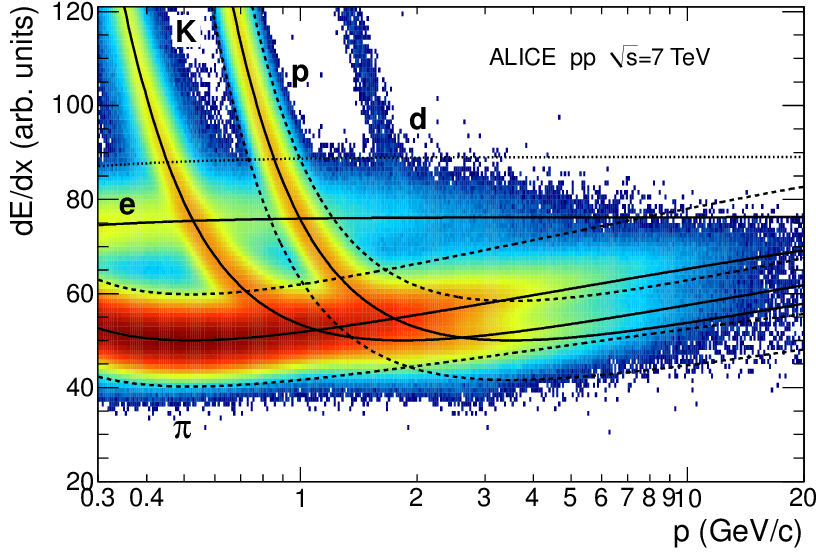
\includegraphics[width=0.7\linewidth]{training&testing/Specific-energy-loss-in-the-TPC.png}
        \caption{ Perdita di energia specifica nella TPC in funzione del momento. Sono riportati anche gli andamenti della Bethe-Bloch per vari tipi di particelle (linee nere continue).}
        \label{fig:BBnellaTPC}
    \end{figure}
   
  
  \subsection{Valutazione delle Variabili Discriminatorie}
  
    L'utilizzo di variabili discriminatorie correlate tra loro generalmente peggiora le performance dell'algoritmo di machine learning sia per quanto riguarda la capacit\`a di selezionare il segnale dal fondo, sia per i tempi necessari per il training e l'applicazione dell'algoritmo.  
    \\Si \`e considerata, perci\`o la correlazione lineare tra le variabili discriminaotrie utilizzate. In figura \ref{fig:correlazInizialeS} e \ref{fig:correlazInizialeB} \`e riportata la correlazione in percentuale tra tutte le variabili discriminatorie utilizzate nel primo set per il training (ovvero i numeri: 3, 4, 5, 7, 8, 9, 10, 11, 12, 13, 14, 15 e 16 dell'elenco sopra riportato) sia per il segnale che per il fondo.
    
    \begin{minipage}{.5\textwidth}%{0.5 cm} 
        \begin{flushleft} \large
        \flushleft
        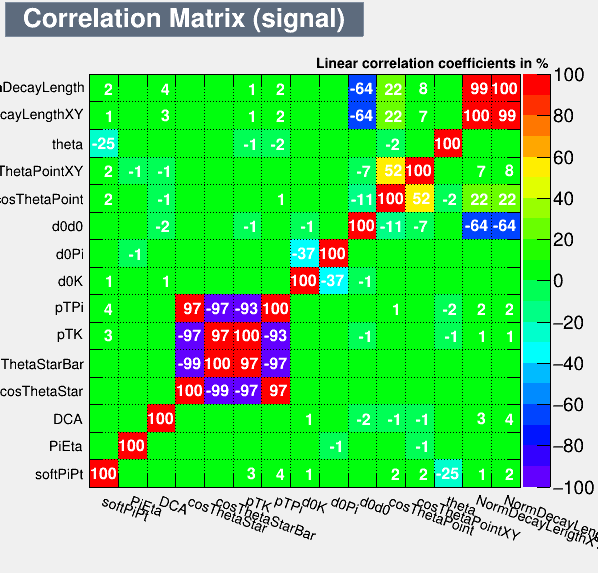
\includegraphics[width=7.5cm]{training&testing/CorrelationMatrixSin.png}
        \captionof{figure}{Correlazione lineare in percentuale tra le variabili discriminatorie considerate inizialmente per il training del segnale (da simulazione Monte Carlo)}
        \label{fig:correlazInizialeS}
        \end{flushleft}
        \end{minipage}
    ~
    \begin{minipage}{0.5\textwidth}
        \begin{flushright} 
        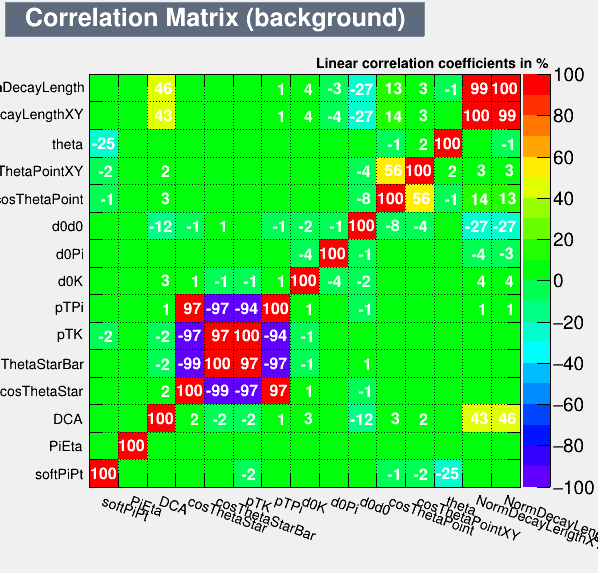
\includegraphics[width=7.5cm]{training&testing/CorrelationMatrixBin.png}
        \captionof{figure}{Correlazione lineare in percentuale tra le variabili discriminatorie considerate inizialmente per il training del fondo (da simulazione Monte Carlo)}
        \label{fig:correlazInizialeB}
        \end{flushright}
    \end{minipage}\\[0.5cm]
    
    Dalle figure \ref{fig:correlazInizialeS} e \ref{fig:correlazInizialeB} si vede che per alcune delle variabili discriminatorie utilizzate nel primo set la correlazione \`e alta e in particolare supera il $50 \%$ per le variabili:
    \begin{itemize}
        \item NormDecayLenght, NormDecayLenghtXY e d0d0 per il segnale
        \item NormDecayLenght, NormDecayLenghtXY e DCA per il fondo 
        \item CosThetaPoint e CosThetaPointXY sia per il segnale che per il fondo
        \item pTpi, pTK, CosThetaStar e CosThetaStarBar sia per il segnale che per il fondo
    \end{itemize}
    
    Si \`e pertanto deciso di non considerare nell'analisi le variabili: NormDecayLenght, CosThetaPoint, pTpi, pTK e CosThetaStarBar.
    
    In figura \ref{fig:correlazFinaleS} e \ref{fig:correlazFinaleB} sono riportate le correlazioni lineari in percentuale per il set modificato di variabili discriminatorie utilizzate per il training, in cui sono state levate le variabili correlate di cui si \`e parlato e sono state aggiunte le variabili relative all'identificazione delle particelle. Il set di variabili \`e composto dai numeri: 3, 7, 8, 9, 10, 12, 13, 14, 16, 17, 18, 19, 20 relativi agli elenchi numerati precedenti.
    \\
    
      \begin{minipage}{.5\textwidth}%{0.5 cm} 
        \begin{flushleft} \large
        \flushleft
        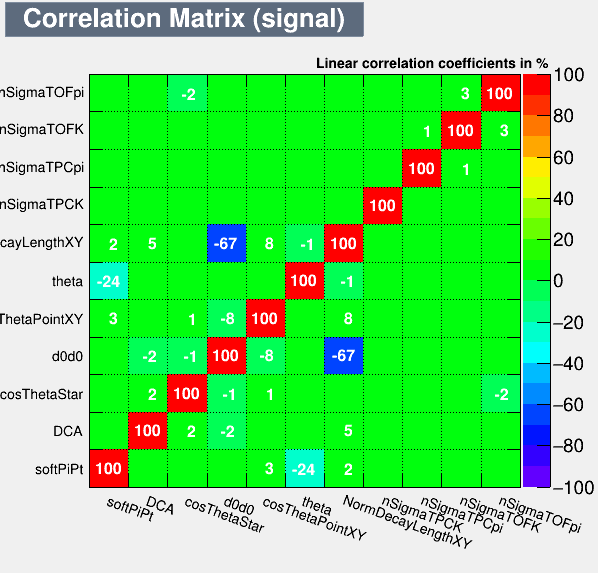
\includegraphics[width=7.5cm]{training&testing/CorrelationMatrixS.png}
        \captionof{figure}{Correlazione lineare in percentuale tra le variabili di taglio considerate per il training finale del segnale (da simulazione Monte Carlo)}
        \label{fig:correlazFinaleS}
        \end{flushleft}
        \end{minipage}
    ~
    \begin{minipage}{0.5\textwidth}
        \begin{flushright} \large
        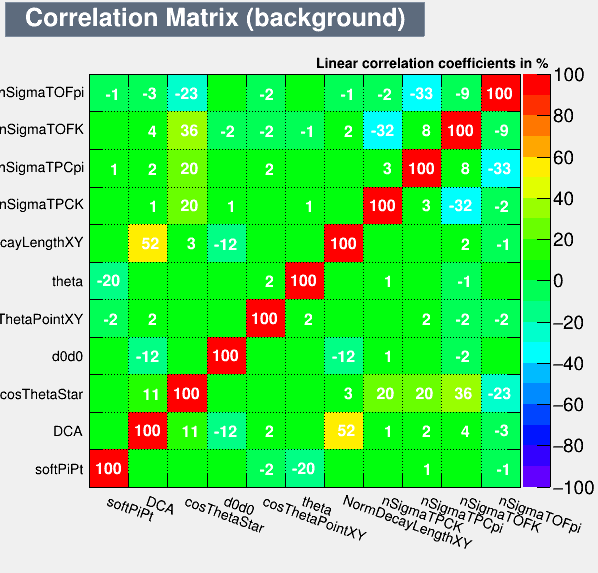
\includegraphics[width=7.5cm]{training&testing/CorrelationMatrixB.png}
        \captionof{figure}{Correlazione lineare in percentuale tra le variabili di taglio considerate per il training finale del fondo (da simulazione Monte Carlo)}
        \label{fig:correlazFinaleB}
        \end{flushright}
    \end{minipage} \\[1.cm]
    
 Come si vede dalle figure \ref{fig:correlazFinaleS} e \ref{fig:correlazFinaleB} la correlazione tra le variabili discriminatorie \`e inferiore al $50 \%$ per tutte le variabili discriminatorie considerate ad eccezione di:
 \begin{itemize}
     \item NormDecaYLenghtXY e d0d0 per il segnale
     \item NormDecayLenghtXY e DCA per il fondo
 \end{itemize}
   
  Quest'ultimo set di variabili indicato \`e quello su cui \`e stata svolta l'analisi finale di cui si riporteranno i risultati nel seguito. 
  
%\section{Training}



\subsection{Campione del training}
Come detto in precedenza per la fase di training del BDT è necessario un insieme di dati di cui sia nota la distinzione tra segnale e fondo. 
\\Per il segnale è stato utilizzato un campione di simulazione Monte Carlo, essendo questo l'unico modo per essere certi di considerare dati relativi alla $D^{*+}$. Per il fondo si sono considerate due opzioni differenti:
\begin{itemize}
    \item dati per il fondo ottenuti da simulazione Monte Carlo ottenuti considerando le combinazioni di due $\pi^+$ e un $K^-$ non relative alla $D^{*+}$
    \item fondo preso dai dati di ALICE, considerando le candidate $D^{*+}$ a destra e a sinistra del picco di segnale della $D^{*+}$. In particolare si sono presi i dati con valori della differenza tra la massa invariante della $D^{*+}$ e della $D^0$: $\Delta M > 147.8 MeV/c^2$  e $\Delta M < 143.0 MeV/c^2$
\end{itemize}

Per gli algoritmi di analisi multivariata, come il BDT, è importante che i dati utilizzati per il training siano il più aderente possibile ai dati da analizzare nella fase di applicazione. Pertanto per il fondo si è scelto di utilizzare i dati di ALICE a destra e sinistra del segnale.
\\In figura \ref{fig:dati_training} è riportata la distribuzione dei dati utilizzati per il training, in cui si vedono i dati da simulazione Monte Carlo per il picco di segnale e i dati di ALICE per il fondo. 

    \begin{figure}[htbp] 
        \centering
        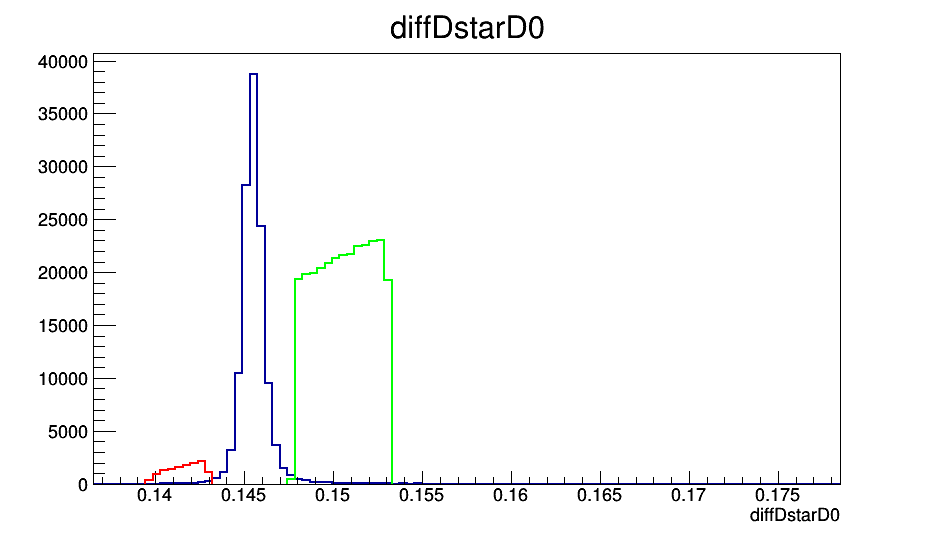
\includegraphics[width=0.9\linewidth]{training&testing/diffDstarD0_training_3_4_ok.png}
        \caption{Dati utilizzati per il training per l'intervallo di $p_T$ [3-4] $GeV/c$, $\Delta M = M(K,\pi,\pi)-M(K,\pi))$ : in rosso il segnale dai dati di simulazione Monte Carlo, in blu il fondo ottenuto dai dati di ALICE}
        \label{fig:dati_training}
    \end{figure}
    
 Nella tabella \ref{Tab:dati_training} si riporta la quantità di dati per il segnale e per il fondo utilizzati per il training in ogni intervallo di $p_T$. 
 
      \begin{table}[H]
		\centering
		\captionof{table}{Dati utilizzati per il training\label{Tab:dati_training}}
		\begin{tabular}{c|c|c}
		    \toprule
		    intervallo $p_T$ [GeV/c]  &   dati training segnale & dati training fondo  \\
            \midrule
            1 - 2  	&  10000   &  100000  \\ 
            2 - 3 	&  30000   &  90000  \\
            3 - 4  	&  30000   &  30000  \\ 
            4 - 5  	&  20000   &  10000 \\ 
            5 - 6  	&  17000   &  4000  \\ 
            6 - 8  	&  20000   &  2800  \\ 
            8 - 12  &  12000   &   900 \\   
			\bottomrule
		\end{tabular}
	\end{table}
	
Gli algoritmi di analisi multivariata hanno bisogno di un grande quantità di dati per il training, così da poter apprendere correttamente le informazioni da utilizzare poi nella fase di applicazione. Si nota che per valori di $p_T > 12  \ GeV/c$ si hanno meno di 500 eventi per il fondo e pertanto si è deciso di non considerare gli intervalli di $p_T$ [12-16] e [16-24] GeV/c. Inoltre, per valori di $p_T < 1 \ GeV/c$ si hanno meno di 500 eventi per il training del segnale, perciò in questa tesi non si considera l'intervallo di $p_T$ [0,1] $GeV/c$.
 
    

\subsection{Scelta dei Parametri del BDT}
Alcuni parametri dell'algoritmo del BDT possono essere variati andando a cambiare le performance dell'algoritmo.
Per valutare le performance dell'algoritmo del BDT si è utilizzata la \textit{ROC-Curve} (Receiving Operating Characteristics Curve) e in particolare l'area sottesa alla ROC-Curve. La ROC-Curve è il grafico della $background rejection$ in funzione della $signal efficiency$. La $background rejection$ è $1 - background efficiency$, la $background efficiency$ è il numero di eventi del fondo selezionati come fondo e la $signal efficiency$ è il numero di eventi segnale selezionati come segnale. Un algoritmo è tanto più efficiente quanto più è alto il valore dell'area della Roc-Curve.
\\Per l'analisi svolta in questa tesi sono stati variati due parametri del BDT:
    \begin{itemize}
        \item \textit{numero di alberi} che compongono la "foresta" del BDT. Come spiegato nel paragrafo \ref{BDT}  il training viene fatto su un grande numero di alberi il cui responso viene unito in un'unica variabile finale. In generale all'aumentare del numero di alberi l'efficienza dell'algoritmo migliora, ma aumenta anche il tempo necessario sia per il training che per l'applicazione del BDT. Si sono fatti alcuni tentativi per cercare un buon compromesso tra le performance dell'algoritmo e il tempo impiegato per analizzare i dati.  Nella tabella \ref{Tab:trees} si riporta il valore dell'area sottesa alla RoC-Curve per alcuni valori del numero di alberi considerati per il training fatto nell'intervallo di $p_T: \  [3-4] \ GeV/c$.
       
        \begin{table}[H]
		\centering
		\captionof{table}{Area sottesa alla Roc-Curve per i rispettivi valori del numero di alberi\label{Tab:trees}}
		\begin{tabular}{c|c}
		    \toprule
		    numero di alberi  &  area Roc-Curve  \\
            \midrule
              50 &   0.940 \\ 
           	 200 &   0.944  \\ 
             300 &   0.945 \\
             850 &   0.947 \\ 
			\bottomrule
		\end{tabular}
	\end{table}
	
	Per l'analisi svolta in questa tesi è stato utilizzato un BDT con 300 alberi.
	
	\item \textit{profondità massima} di ciascun albero del BDT. La profondità di un albero è il numero di livelli di cui è composto l'albero, ovvero di diramazioni. Come per il numero di alberi, in generale, se si aumenta la profondità massima migliorano le performance dell'algoritmo, ma aumenta il tempo necessario per l'analisi dei dati.
	Nella tabella \ref{Tab:profondità} è riportata l'area sottesa alla Roc-Curve per i valori di profondità considerati, per il training fatto con 300 alberi nell'intervallo di $p_T: \ [3,4] \ GeV/c$.
	
	\begin{table}[H]
		\centering
		\captionof{table}{Area sottesa alla Roc-Curve per i rispettivi valori della profondità degli alberi\label{Tab:profondità}}
		\begin{tabular}{c|c}
		    \toprule
		    profondità  &  area Roc-Curve  \\
            \midrule
           	 2 &   0.924  \\ 
             3 &   0.945 \\
             4 &   0.947 \\ 
			\bottomrule
		\end{tabular}
	\end{table}
	Si è scelto di utilizzare alberi con profondità 3 nell'analisi svolta in questa tesi.
    \end{itemize}

\section{I risultati del Training}

Una volta identificate le variabili discriminatorie scorrelate, la configurazione del BDT e il campione da usare come segnale e fondo si è proceduto con il training. In questa sottosezione si considerano i risultati ottenuti dal training del BDT. 
\\Come detto in precedenza, per valutare le performance del BDT si considera la Roc-Curve. In figura \ref{fig:RocCurve} è riportata la Roc-Curve relativa la training del BDT con 300 alberi con profondità massima 3 per l'intervallo di $p_T$ [3-4] $GeV/c$. 

    \begin{figure}[htbp] 
        \centering
        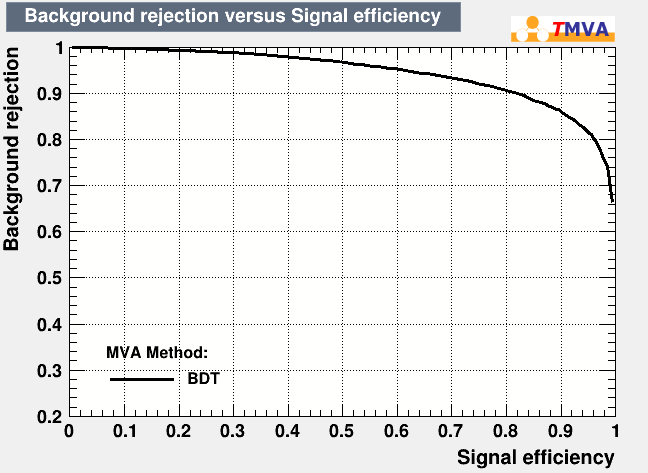
\includegraphics[width=0.7\linewidth]{training&testing/RocCurve.png}
        \caption{Grafico della ROC-Curve relativa al training del BDT con 300 alberi e profondità massima 3 per l'intervallo di $p_T$ [3,4] $GeV/c$}
        \label{fig:RocCurve}
    \end{figure}
    
    
Un'altra grandezza da considerare è la distribuzione dei dati in funzione del classifier output. Le variabili discriminatorie sono combinate tra loro per determinare un'unica variabile, che permette di differenziare il segnale dal fondo, e che nel resto del capitolo sarà chiamato \textit{BDT response}. Il grafico in figura \ref{fig:BDTresponse} mostra la distribuzione del BDT response per il segnale (blu) e per il fondo (rosso). Nella figura si vede che le distribuzioni del segnale e del fondo sono ben distinte e che solo una parte del fondo si sovrappone al segnale. 

    \begin{figure}[htbp] 
        \centering
        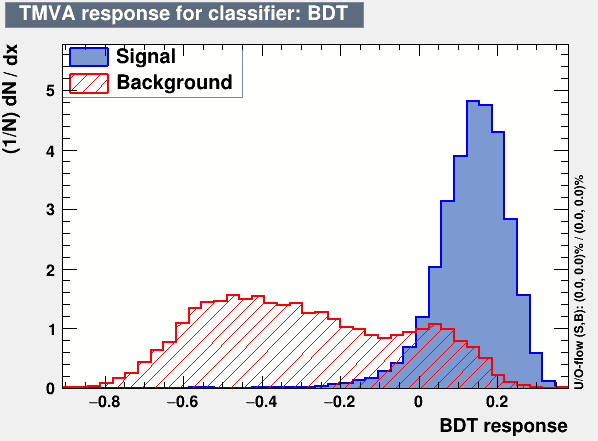
\includegraphics[width=0.7\linewidth]{training&testing/BDTresponsetest.png}
        \caption{Distribuzione del BDT response del training con 300 alberi e profondità massima 3. In blu i dati relativi al segnale e in rosso quelli relativi al fondo}
        \label{fig:BDTresponse}
    \end{figure}
    
Se confrontiamo la distribuzione dei dati in figura \ref{fig:BDTresponse} e quella rispetto alle variabili di taglio in figura \ref{fig:variabilitaglio}, si nota facilmente quanto la differenza tra la distribuzione del fondo e del segnale sia aumentata considerando il BDTresponse, piuttosto che le grandezze fisiche delle variabili di taglio. Questo è proprio il vantaggio offerto dall'analisi multivariata e nel caso specifico dall'algoritmo del BDT.
\\L'\textit{efficienza del segnale} del BDT è il numero di eventi segnale che sono stati classificati dall'algoritmo come segnale, l'\textit{efficienza del fondo} è il numero di eventi del fondo classificati come fondo.
Si è considerata anche la significatività, che è definita come:
    \begin{equation}
        sign \ = \ \frac{segnale}{\sqrt{segnale + fondo}}
    \end{equation}
Sia l'efficienza del segnale che quella del fondo, che la significatività variano in base al valore di taglio scelto per la variabile BDT response. Il valore di taglio del BDT response è il valore scelto come limite per separare il segnale dal fondo.
\\In figura \ref{fig:efficienza} sono riportati gli andamenti dell'efficienza del segnale (in verde), del fondo (in blu) e della significatività (in verde) per il training fatto sull'intervallo di $p_T$ [3,4] $GeV/c$.

    \begin{figure}[htbp] 
        \centering
        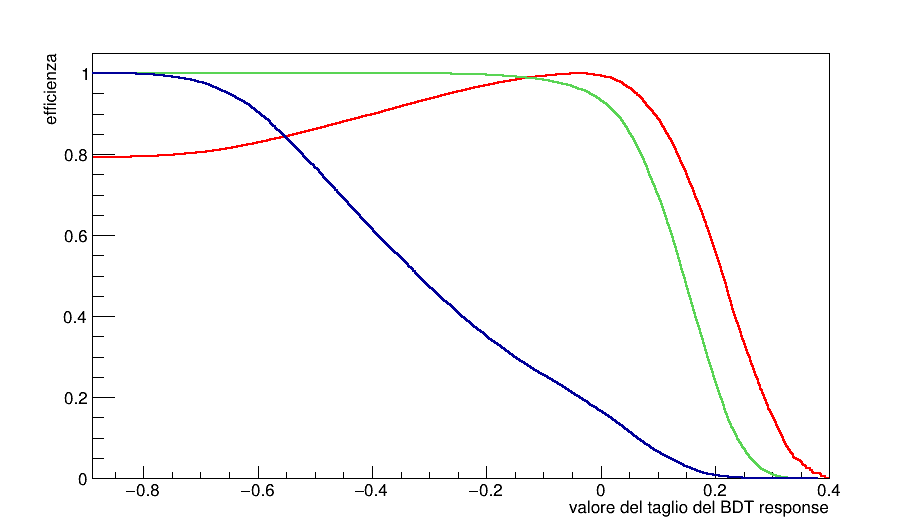
\includegraphics[width=0.7\linewidth]{training&testing/eff_signok.png}
        \caption{Efficienza del segnale in verde, del fondo in rosso e significatività in rosso, per il training dell'intervallo di $p_T$ [3,4] $GeV/c$ in funzione del valore del taglio applicato sulla variabile BDT response}
        \label{fig:efficienza}
    \end{figure}



    
  %Inoltre, si deve considerare che all'aumentare del $p_T$ il picco di segnale nella distribuzione dei dati di ALICE rispetto alla variabile $diffD^{*+}D^0$ diventa sempre più evidente e più facilmente individuabile anche con un'analisi che non utilizza metodi multivariati. Pertanto non è stata continuata l'analisi dati anche per valori di $p_T \ > \ 12 \ Gev/c$. 



\section{Testing} \label{testing}
    Una parte dei dati generati dalla simulazione Monte Carlo non sono stati utilizzati per il training e vengono utilizzati per la fase di verifica del training stesso, detta \textit{testing}. 
    \\In questa fase si vuole controllare che non ci sia stato \textit{overtraining} durante la fase di training, ovvero che il BDT si sia adattato eccessivamente al campione di dati del training e non sia più descrittivo del fenomeno fisico che si vuole considerare nella  sua generalità. e non c'è stato overtraining, ci si aspetta che la distribuzione del BDT response sia la stessa per i dati del training e quelli del testing. 
    \\In tabella \ref{Tab:test} è riportata la quantità di dati da simulazione Monte Carlo utilizzata per il testing per ogni intervallo di $p_T$ considerato.
    
    \begin{table}[H]
		\centering
		\captionof{table}{Dati utilizzati per il testing\label{Tab:test}}
		\begin{tabular}{c|c|c}
		    \toprule
		    intervallo $p_T$ [GeV/c]  &   dati testing segnale & dati testing fondo  \\
            \midrule
            1 - 2  	&  3165   &  37853  \\ 
            2 - 3 	&  11560   &  26498  \\
            3 - 4  	&  14395   &  14743  \\ 
            4 - 5  	&  13292   &  6090 \\ 
            5 - 6  	&  5868   &  1076  \\ 
            6 - 8  	&  6301   &  719  \\ 
            8 - 12  &  5589   &   464 \\   
			\bottomrule
		\end{tabular}
	\end{table}
    
    \\In figura \ref{fig:testing_3_4} è riportata la distribuzione del BDT response per i dati del training e del testing per l'intervallo di $p_T$ [3,4] $GeV/c$. Dalla figura si vede che le distribuzione per il training e per il testing coincidono completamente entro gli errori.
    
    
    \begin{figure}[htbp] 
        \centering
        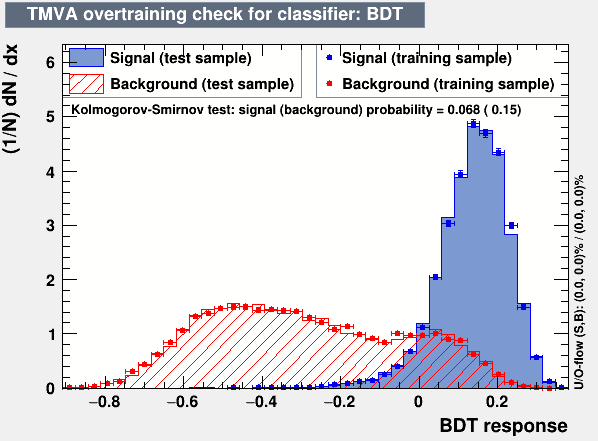
\includegraphics[width=0.7\linewidth]{training&testing/overtraining_3_4.png}
        \caption{Distribuzione del BDT response per il training (punti e relativi errori) e per il testing (rettangoli) per il bin di $p_T$ [3,4] $GeV/c$, in rosso i dati del fondo e in blu quelli relativi al segnale}
        \label{fig:testing_3_4}
    \end{figure}
 
    In figura \ref{fig:testing_6_8} si vede la distribuzione del BDT response per i dati del training e del testing per l'intervallo di $p_T$ [6,8] $GeV/c$. Si vede che le distribuzioni per il training e per il testing sono compatibili per la maggior parte dei valori del BDT response. 
 
    \begin{figure}[htbp] 
        \centering
        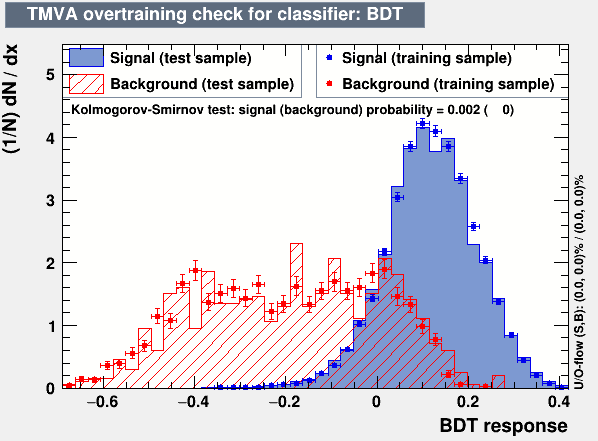
\includegraphics[width=0.7\linewidth]{training&testing/overtraining_6_8.png}
        \caption{Distribuzione del BDT response per il training (punti e relativi errori) e per il testing (rettangoli) per il bin di $p_T$ [6,8] $GeV/c$, in rosso i dati del fondo e in blu quelli relativi al segnale}
        \label{fig:testing_6_8}
    \end{figure}
 
    I grafici \ref{fig:testing_3_4} e \ref{fig:testing_6_8} mostrano che non c'è stato overtraining, pertanto si può procedere con l'analisi dei dati.




\section{Scelta dei valori di taglio}

Ottenute le distribuzioni del BDT response e gli andamenti delle efficienze e della significatività per i vari intervalli di $p_T$ considerati, si sono individuati i valori di taglio del BDT response. In base ai valori di taglio si discriminerà tra segnale e fondo nella fase di applicazione del BDT. 
\\Per scegliere il valore di taglio della variabile di output del BDT per separare segnale e fondo si sono provate diverse opzioni:
    \begin{itemize}
    \item il punto di massimo della significatività
    \item il punto in cui la curva dell'efficienza del segnale e la curva della significatività si incontrano. Questo è stato fatto per cercare di avere un buon compromesso tra la significatività e la quantità di segnale selezionata. 
    \end{itemize}
    
Per scegliere il valore del taglio migliore si sono considerati i risultati della fase di applicazione del BDT. Si è scelto di utilizzare come valore del taglio il punto di incontro tra la curva dell'efficienza e della significatività.
\\In tabella \ref{Tab:tagli} si riportano i valori del taglio scelti per ogni intervallo di $p_T$.

\begin{table}[H]
		\centering
		\captionof{table}{Valori del taglio del BDT response\label{Tab:tagli}}
		\begin{tabular}{c|c}
		    \toprule
		    intervallo di $p_T$ [GeV/c]  &  valore del taglio  \\
            \midrule
           	1 - 2  	&    0.049   \\ 
            2 - 3 	&    0.045  \\ 
            3 - 4  	&    0.031  \\ 
            4 - 5  	&    0.027  \\ 
            5 - 6  	&    0.031  \\ 
            6 - 8  	&    0.034  \\ 
            8 - 12  &    0.105  \\   
			\bottomrule
		\end{tabular}
	\end{table}

%Nell'utilizzare i grafici di efficienze e significatività per la scelta del valore di taglio è stato fondamentale aver considerato un rapporto segnale-fondo molto basso (10:1000), questo perchè nei dati di ALICE abbiamo che gli eventi segnale sono molti meno degli eventi fondo. In tal modo anche i risultati del training del BDT e le curve di efficienze e significatività sono più aderenti ai dati di ALICE.

  %  \begin{figure}[htbp] 
   %     \centering
  %      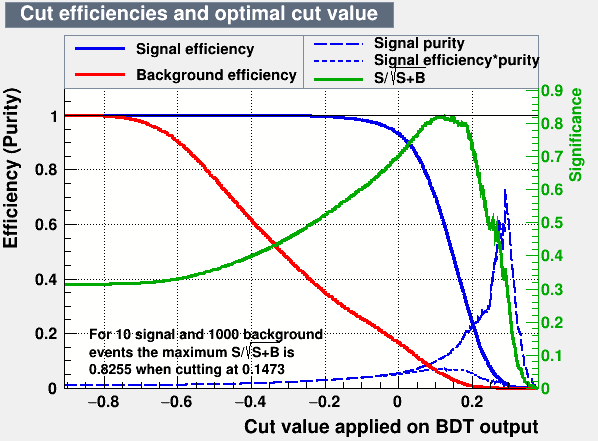
\includegraphics[width=0.7\linewidth]{training&testing/effBDT/effBDT_rapp_3_4.png}
  %      \caption{Grafico dell'efficienza del segnale in blu, efficienza del fondo in rosso e significatività in verde, al variare del valore del taglio scelto per la BDTresponse per il bin di $p_T$ [3,4]. Il rapporto tra segnale e fondo è di 10:1000 . Gli andamenti sono relativi al training con 300 alberi e profondità massima 3
   %     }
   %     \label{fig:effBDT_10_1000}
   % \end{figure}
  
  
  
  %modificare
 %Per i bin di $p_T$ più alti i grafici della significatività diventano sempre meno lineari. probabilmente a causa del diminuire della quantità di dati utilizzata per il training, pertanto in alcuni casi è stato scelto un valore di taglio più alto rispetto a quello del metodo precedentemente indicato.
